% !TeX root = ../main.tex
% Add the above to each chapter to make compiling the PDF easier in some editors.

\chapter{Background}\label{chapter:background}

\section{Sensor}

Our modern world us infused with sensors. We use sensors in everyday life concisely or subconsciously. From our smartphone, cars to the state of the art medical equipment, mars roves has a variety of uses of sensors. Although when the term sensor comes up we think about mostly mechanical sensors, such as touchscreen in our smartphone or the fire detection sensor, sensors can be not only mechanical but also chemical, bio, and other variety of types.

These sensors are collecting data every moment in our modern world. For example, our buses, trains, planes, and ships are using GPS to navigate around the world. We are using our smartphone which has a variety of sensors working together like the camera, touch sensors, gyro, GPS, and proximity sensor. They are working continuously in the background and processing data to make our life a  little bit easier. Now we can sense and track out heartbeat just using a wristwatch.

The use of smart sensors in our homes, offices, shopping malls, cars is getting bigger and bigger nowadays. All modern means of transport such as cars, buses, trains are using sensors to create a more comfortable transport experience. For instance, proximity sensors for better parking experience, crash prevention. If we talk about air transportation, the impact of sensors is even more important and critical for instance temperature, air pressure sensors. A single failure of any of these sensors could lead to deadly outcomes with fatality. The list goes on when it comes to the use of sensors and their impacts on our life

n the broadest definition, a sensor is a device that can  monitor the environment that its designed for. A sensor is a device or an integrated system of devices that senses and responds to certain types of environmental inputs. Light, heat, movement, moisture, pressure, or any of a number of other environmental phenomena could be the specific input. The output is usually a signal converted for reading or continuing processing to a human-readable display at the point of the sensor or electronically transmitted over a network. Due to the different needs, the properties of sensors were changed a lot over time. The need enabled intelligent and intelligent sensors to be created. The advent of intelligent sensors led to the development of microcontrollers used everywhere. The smart sensors have allowed us to interface with other devices and make them work together as one device.


\subsection{Sensor Types}

As we mentioned before, sensors can be many types, It can be categorized depending on their purpose or depending on how they are made. There are various sensor classifications created by different writers and specialists. An expert in the subject can already use the following sensor classification, but it is an extremely simple sensor classification. They are divided into active and passive in the first classification of the sensors. Active sensors are those that require a power signal or an external excitation signal. On the other hand, passive sensors do not require an external power signal and generate an output response directly. Analog and optical sensors are the final grouping of the sensors. Analog capabilities generate an analog output.

We have a long list of sensors, which we use in our everyday work. If we want to speak briefly about them, we can hardly cover each sensor. We will discuss a few of them which is somewhat related to our work. The sensor mention below are regardless of their classes, they are a mix of digital, analog, active sensors.

\subsubsection{Temperature sensors or thermal sensors}

This system collects temperature information from a system and transforms it into a way that another system or individual can understand. Mercury in a glass thermometer is the simplest example of a temperature sensor. Mercury expands in the glass and contracts to rely on temperature changes. The external temperature is the source factor for measuring the temperature. In order to calculate the temperature, the spectator measures the location of mercury. Two basic temperature sensors are available:

\begin{figure}[h]
  \centering
    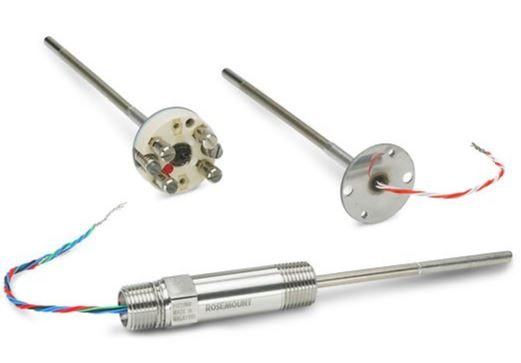
\includegraphics[width=0.8\linewidth]{figures/tempSensor.jpg}
    \caption{A typical temperature sensor.}
    \source {emerson.com}
\label{fig:tempSensor}
\end{figure}


\begin{itemize}
 \item Contact sensors – This type of sensor requires physical direct contact with the sensed object or media. They monitor solids, liquids, and gas temperatures across a broad range of temperatures.
 \item  Non-contact Sensors – No physical contact with the object or the media is required for this type of sensor. They monitor non-reflective solids and liquids, but because of natural transparency, they are not useful for gasses. These sensors use the Law of Plank for temperature calculation. This law covers heat radiated from the heat source for temperature measurements.

\end{itemize}


\subsubsection{Sonar sensors}


Sonar sensor: As the name suggests, the Sonar sensor also known as Ultrasonic sensor works based on an ultrasonic pulse time calculation to measure distance.


\begin{figure}[h]
  \centering
    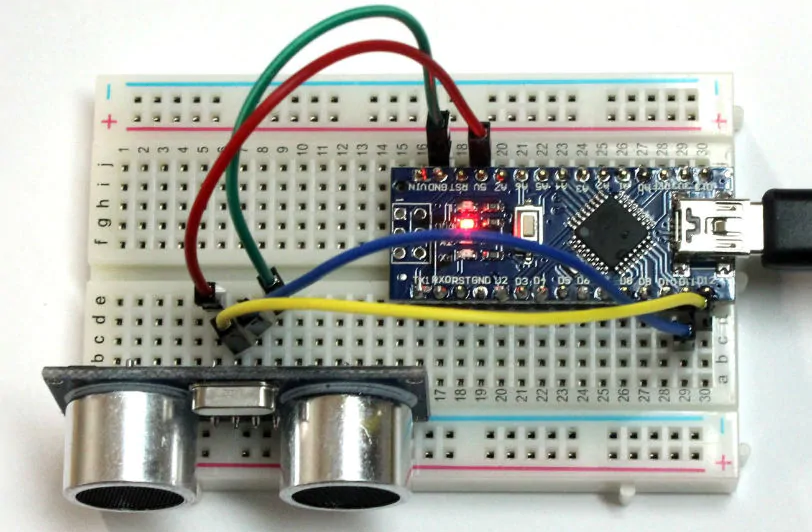
\includegraphics[width=\linewidth]{figures/sonarSensor.png}
    \caption{A sonar sensor combined with microcontroller}
    \source {arrow.com}
\label{fig:sonarSensor}
\end{figure}


To measure the specific distance from the sensor, this can be calculated based on this formula \cite{sonar1}:

Distance = 1/2 T x C 


where T is time and C is the spped of sound in specific temparatuer of earth environment. At 20$^{\circ}$ C (68$^{\circ}$ F), the speed of sound is 343 meters/second (1125 feet/second), but this varies depending on temperature and humidity.


\subsubsection{IR Sensors}

These types of sensors sense the infrared light. In general, all objects on the infrared ( IR ) spectrum emit thermal radiation. That kind of radiation that is not visible to the human eye is measured by the infrared sensor. The biggest advantage of the IR sensor is that it uses very cheap and available and very easy to use. One of the major drawbacks of these sensors is that it pruned to background noise.

\begin{figure}[h]
  \centering
    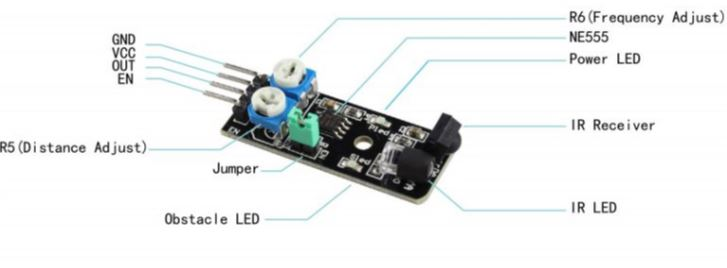
\includegraphics[width=\linewidth]{figures/irSensor.jpg}
    \caption{An IR sensor architecture}
    \source {ram-e-shop.com}
\label{fig:irSensor}
\end{figure}


The working of IR sensor and sonar sensor is similar, where the sonar sensor emits soundwave and have a receiver for the sound wave the IR use infrared light instead of sound. 

\begin{figure}[h]
  \centering
    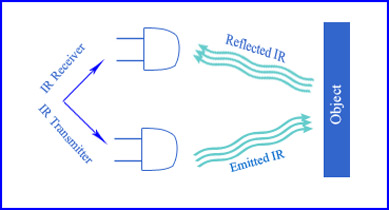
\includegraphics[width=0.5\linewidth]{figures/irSensorWork.jpg}
    \caption{Working principal of an IR sensor}
    \source {engineersgarage.com}
\label{fig:irSensorWork }
\end{figure}


\subsubsection{UV Sensors}

Such sensors measure the intensity or strength of the UV radiation incident. It has a longer wavelength than x-rays but is also shorter than the visible radiation. For robust ultraviolet sensing, an active material called polycrystalline diamond is used. UV sensors can detect exposure to ultraviolet radiation from the environment.


\begin{figure}[h]
  \centering
    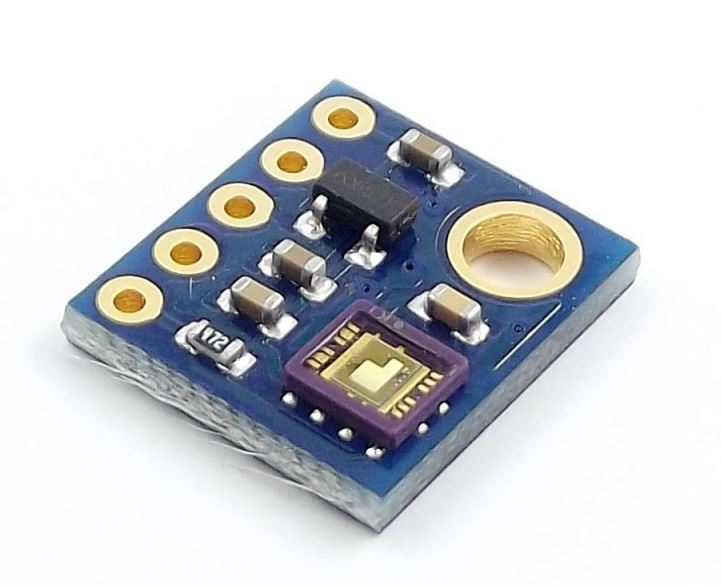
\includegraphics[width=0.5\linewidth]{figures/uvSensor.jpg}
    \caption{UV sensor}
    \source {roboticsbd.com}
\label{fig:uvSensor }
\end{figure}


The UV sensor recognizes one energy signal type and transmits different energy signals. They are directed to an electric meter to observe and record these output signals. The output signals are transmitted for the generation of graphs and reports to a software-based computer through an analog-to-digital converter ( ADC).


\subsubsection{Touch Sensor}

A touch sensor functions as a variable resistor according to the position of the touch. As seen in figure \ref{touchSensorWork}

\begin{figure}[h]
  \centering
    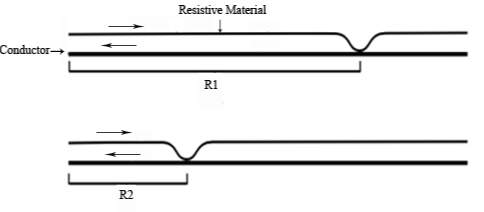
\includegraphics[width=0.5\linewidth]{figures/touchSensorWork.png}
    \caption{Working mecanism of a touch sensor}
\label{fig:touchSensorWork }
\end{figure}

A touch sensor made of a substance that is absolutely conductive such as copper Isolated material for the spacing of foam or plastic or material which is partly conductive.
The way the touch sensor works is that the surface is partly conductive and opposes the present flow. The key concept of the linear position sensor is that when the length of this material, to be traveled by the current, is greater, the current flow is contrasted. The resistance of the material is therefore varied by adjusting the location at which it comprises the substance that is completely conductive.

\subsubsection{Global Positioning System (GPS) sensor}

We use the GPS sensor almost every day in our life, mostly via our phone or in our car, the GPS sensor is used to navigate around the world.

A minimum of 24 operational satellites orbit over 12,000 kilometers above ground at any given time. The locations of the satellites will always include up to 12 satellites in the sky above your location. The primary function of the 12 visible satellites is to relay radio frequency (1.1-1.5 GHz) information back to earth. A soil-based receiver or GPS module may measure its location and time with this information and other mathematical details. \cite{misra2006globa}



\subsubsection{LiDAR}

Lidar is an analogy for "light detection and ranging." The device uses eye-safe laser beams to produce a 3D view of the surroundings being scanned.


\begin{figure}[h]
  \centering
    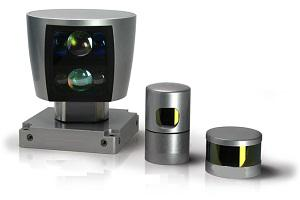
\includegraphics[width=0.5\linewidth]{figures/lidarSensor.jpg}
    \caption{A Lidar device used for automotive}
    \source {Automotive Lidar Sensor Market 2017 - Leddar, Quanergy}
\label{fig:lidarSensor}
\end{figure}


A typical lidar sensor absorbs the ambient atmosphere with pulsed light waves. Such pulses rebound and come back to the sensor. To calculate the distances traveled, the sensor takes time for every pulse to return to the sensor. This procedure is repeated millions of times per second and creates a precise 3D environmental map in real-time. This chart can be used for secure surfing by an onboard computer.
Lidar is mostly used for advance autonomous systems to measure its surrounding environment.


\subsubsection{Gyroscope sensor}


A device that senses angular velocity is gyro sensors, also known as angular rate sensors or angular velocity sensors.  Gyroscopes in consumer électronics were not only found in compasses, ships, computer pointing instruments, etc.

\begin{figure}[h]
  \centering
    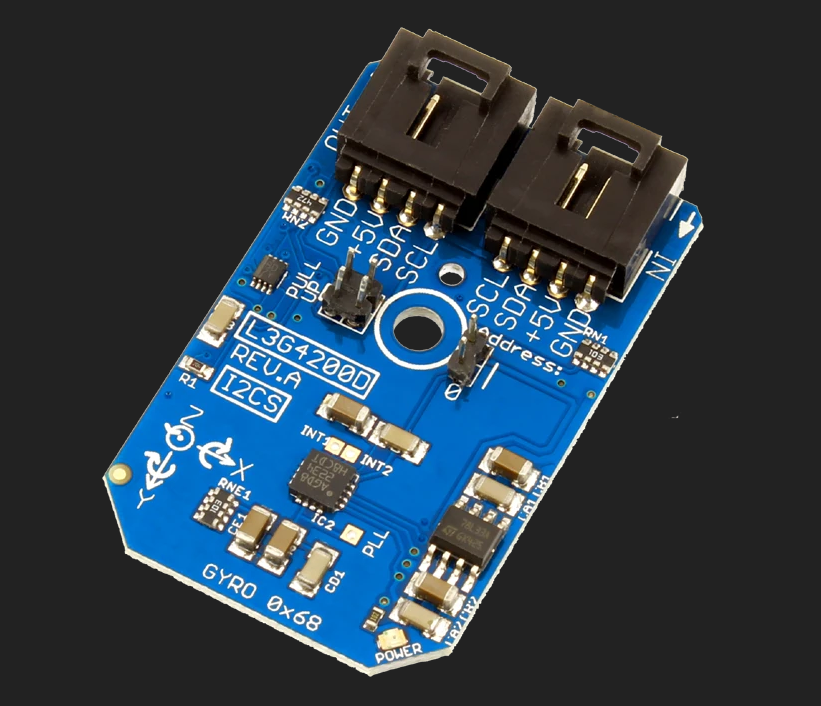
\includegraphics[width=0.5\linewidth]{figures/gyroSensor.png}
    \caption{An MMSE gyroscope}
    \source {controleverything.com}
\label{fig:gyroSensor}
\end{figure}

Since the gyroscope allows orientation and rotation to be measured, designers have combined them with modern technology. The gyroscope technology has made it possible to detect the movement inside a 3D world more reliably than the previous lone accelerometer on most smartphones. Gyroscopes are also paired with accelerometers for better direction and motion sensing in consumer electronics. The gyroscopes inside smartphones don't have wheels and gimbals such as the conventional mechanical ones in an old aircraft, they are MEMS (Micro-Electro-Mechanical Systems)  gyroscopes instead.



\subsubsection{Accelerometer sensor}



It can be used for the measurement of the acceleration exerted on the sensor, as its name implies. The acceleration is usually performed in two or three components of the axis-vector, which make up the acceleration. \cite{FERNANDEZ20138} There are a few uses of Accelerometers, remote controls for videos, smartphones, etc. Accelerometer usually combined with a Gyroscope for better sensing. Accelerometers give us two data types: Static force used on the sensor due to gravity detection in the direction of orientation and  Sensor strength, acceleration to motion, force detection

\begin{figure}[h]
  \centering
    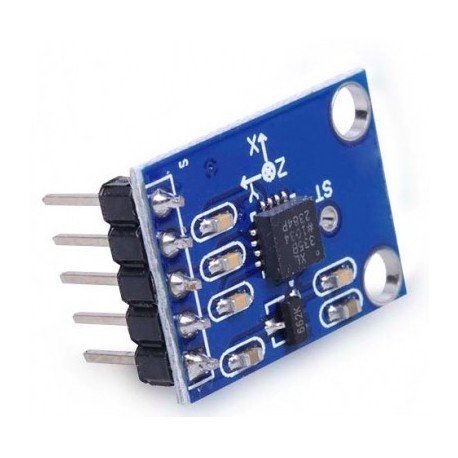
\includegraphics[width=0.5\linewidth]{figures/accSensor.jpg}
    \caption{An electronic accelerometer sensor}
    \source {nuttyengineer.com}
\label{fig:accSensor}
\end{figure}



\subsubsection{Smart Sensors}

Due to the different needs, the sensor characteristics were adjusted a lot over time. The needs allowed intelligent and intelligent sensors to be developed. The IEEE 1451 standard defines smart sensors as a physical device or a combination of sensors with physical connectors for communication with processor and data network. \cite{5739775}.

Fig (smartSensorStructure) source cite [5739775]
\begin{figure}[h]
  \centering
    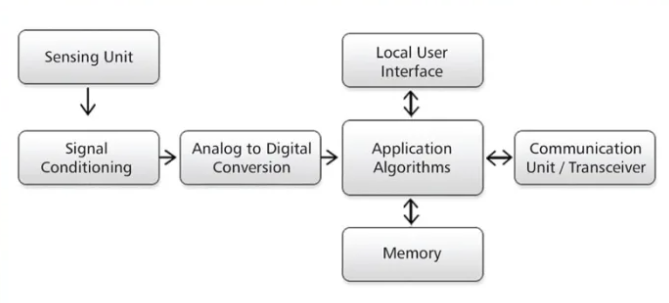
\includegraphics[width=\linewidth]{figures/smartSensorStructure.png}
    \caption{ Smart sensor building blocks }
    \source {Premier Farnell Ltd}
\label{fig:smartSensorStructure}
\end{figure}


The advent of smart sensors contributed to the development of microcontrollers used all over the world. Because of the intelligent sensors, interfacing and working with other peripherals as a single device was possible.
These smart sensors allow us to reduce data volume for communication with the main processor and made faster communication possible. It also reduced power consumption because multiple sensors are used together that use the same processing unit. The major benefit of these smart sensor is that they are typically small and very easy to integrate with other systems even with other sensors.

Here come the uses of IMU (Inertial Measurement Units). In the next section, we describe the properties of an IMU.


\subsection{IMU (Inertial Measurement Units)}
As our goal is to use IMU as our main sensor to collect data for acquiring objects position and orientation, this is our principal sensor to study. An IMU is typically a combination (Accelerometer, Gyroscope, Magnetometer) of sensors working together.
In this chapter, we will discuss the IMU, how its functions, its general structure, and the use cases.

\subsubsection{General structure}

The IMU typically consists of 3 individual sensors Accelerometer, Gyroscope, and a Magnetometer. Sometimes it comes with only an Accelerometer and Gyroscope. The Accelerometer, Gyroscope, and a Magnetometer provides the data of acceleration and velocity, orientation and angular velocity, gravitational forces respectively. This typically gives us the 9 axes of measurement on the other hand the IMU consist of only Accelerometer and Gyroscope provide 6 axes of measurement.
Early days the size of IMU was considerably larger compared to the current IMUs. Its because those are made mechanically but thanks to the MEMS or Micro-Electro-Mechanical Systems that are made possible to make these sensors electronically it's miniaturized the size considerably. \cite{MEMS}.
This helps us to integrate with other microcontrollers or microprocessors like Arduino or Raspberry Pi. Due to its miniature of size sometimes the IMUs are also known as MIMU (Miniature Inertial Measurement Units) \cite{2018233}

\begin{figure}[h]
  \centering
    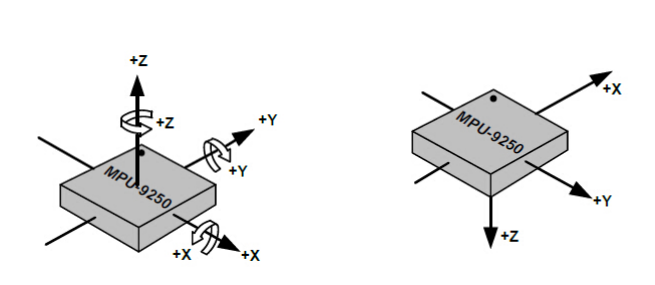
\includegraphics[width=\linewidth]{figures/imuAG.png}
    \caption{ An IMU with 6DoF workiks with a magnetometer for 9DoF }
    \source {Stanford.edu lecture 9 of EE267: Virtual Reality S2020}
\label{fig:imuAG}
\end{figure}


\subsubsection{Working principal of IMU}
The main purpose of IMU is to measure and objects pose relative to its inertial space. Acceleration and angular speed are based on inertial principles are measured.

Accelerometers calculate in a particular direction linear acceleration. An accelerometer can be also used as a downward force to measure gravity. Integrating acceleration once shows a velocity estimate, and integrating again provides you with a position estimate.


\begin{equation}
f^{b}=R^{b n}\left(a_{i i}^{n}-g^{n}\right)
\end{equation}


Although accelerometers can measure linear acceleration, they are unable to measure orientation or rotational motion. Nevertheless, gyroscopes measure angular velocities along three axes: pitch (x-axis), roll (y-axis), and yaw (z-axis). While a gyroscope does not have an initial frame of reference (like gravity), for measuring angular position, you can combine its data with data from an accelerometer. Gyroscope data output angular velocity (deg/s).

The gyroscope measures the angular velocity of the body frame with respect to the inertial frame, expressed in the body frame \cite{ROS}, denoted by $\omega $. This angular velocity can be expressed as

\begin{equation}
\tilde{\omega}=\omega+b+\eta
\end{equation}

The estimated orientation can be obtained by integrating these angular velocities. We can also use Taylor series to measure discrete-time approximation of integration

%\begin{equation}{\theta}_{\text {gyro}}^{(t)}={\theta}_{\text {gyro}}^{(t-1)}+\tilde{{\omega}} \Delta t\end{equation}

Using 3 Gyro and Accelerometer we can obtain an estimated pose of the object in 3D space.
The working principle of a single unit of IMU can be seen in the figure \ref{fig:imuWP}


\begin{figure}[h]
  \centering
    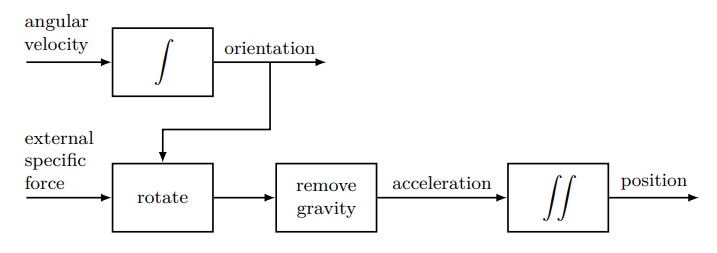
\includegraphics[width=\linewidth]{figures/imuWP.png}
    \caption{ working principle of a single unit of IMU }
    \source {Stanford.edu lecture 9 of EE267: Virtual Reality S2020}
\label{fig:imuWP}
\end{figure}







\section{Sensor fusion}

\subsection{Need of sensor fusion}

First, we have to ask our selves why we need to do sensor fusion if we can get the pose of an object from a single IMU as we can see in the calculation from the previous section {ref section}. But the real-world situation is not an ideal situation. This will only work when there is no bias and no noise but which is unrealistic in the real world. Even if the bias is known and without any noise will have drift from integration. 
For example, the magnetometer which generally works with earth's magnetic pole will have different biases and drift in different places on earth. 
For these reasons, one sensor is not suitable to use for a particular purpose. We need to use multiple sensors in a different formation for that specific purpose to get better accuracy. 
Research shows that there number of the sensor the more number of accuracy you can get. [Chapter 1.1 of your "Instrument Engineers' Handbook," Volume 1 (5th Edition):]
In our situation, we are working with IMU sensors, previous research shows that if we use more IMU we get better accuracy [get cite from adnane]
Now we established that we need more sensors to get better accuracy. But it's not as simple as its sounds, we can not simply get the sensor data and add them together to get the result. To do that we need sensor fusion. Now let's take a look what is sensor fusion.



The benefits of sensor fusion over single source are
the following [Elmenreich, 2001]:
\begin{itemize}
 \item Reliability: Using multiple sensor sources introduces more resilience to partial sensor failure, which leads to greater redundancy and reliability.
 \item Extended spatial coverage: Each sensor may cover different areas. Combining the covered areas will lead to a greater overall coverage of surrounding
environment and accommodate sensor deprivation.
 \item Extended temporal coverage: Each sensor may update at different time intervals, and thus interpolated sensor updates can be joined for increased tem
poral coverage and decreased sensor deprivation.
 \item Increased Confidence: Combining sensor data will provide increased confidence by providing measurements resilient to the uncertainties in any particular
sensor based on the combined coverage and error mitigation of all sensors. \item  Reduced Uncertainty: Given the resilience of multiple sensors to the specific uncertainty of any one, the overall uncertainty of the perception system can be
drastically reduced using sensor fusion.
 \item Robustness against noise: Multiple sensor sources can be used to determine when any one sensor has encountered noise in order to mitigate influence of
noise in the system.
 \item Increased Resolution: Multiple sensor sources can be used to increase the resolution of measurements by combining all observations.
\end{itemize}
According to [Rao, 2001], sensor fusion can yield results that outperform the measurements of the single best sensor in the system if the fusion function class satisfies a
proposed isolation property based on independently and identically distributed (iid)
samples. The fusion function classes outlined that satisfy this isolation property
are linear combinations, certain potential functions and feed-forward piecewise linear
neural networks based on minimization of empirical error per sample.

\subsection{What is sensor fusion}




People tend to think that sensor fusion and sensor integration is the same thing but these two are very different terms for acquiring multiple sensor data. Sensor fusion does not necessarily mean combining multiple sensors together since multiple sensors can be sensed and measured by one sensor, and then the data can be combined together [sensor 2].

Sensor fusion takes data from multiple sensors and fuses them to represent as one for better accuracy.
In simple terms,  Sensor fusion is the act of combining data acquired from two or more sensors sources such that the resulting combination of sensory information provides a more certain description of factors observed by the separate sensors than would be if used individually{cite emirech 2001}

The figure below shows a model of sensor fusion.
fig. modelsf

\begin{figure}[h]
  \centering
    \includegraphics[width=\linewidth]{figures/modelsf.png}
    \caption{ Block model diagram of sensor fusion }
\label{fig:modelsf}
\end{figure}



Sensor fusion is applicable in many applications involving
Usage of the various inference and control sensors. Examples of clude intelligent and automated applications such as automotive driver assistance systems, autonomous robotics, and robotics manufacturing [Elmenreich, 2007]. Methods of sensor fusion attempt to overcome many of the problems already present in sensors. Various important advantages can be derived from fusion sensor systems over single or disparate sensor sources.







\section{Types of sensor fusion}




Several researchers and firms built their own models of sensor fusion systems for specific purposes. Many of these systems in the automotive and robotics sectors are well known and widely used in practice. We can classify sensor fusion in many types based on their model, input-output, architecture. In basic, we can categorized sensor fusion in 2 types based on the algorithme or matmatical model it use. The analytical approach or probabilistic approach and a machine learning approach. We will discuss both types in the following section.



\subsection{Analytical approach}

In the analytical or probabilistic approach of the sensor fusion model, we try to determine the best output estimation of multiple sensors data as a single output. For example, there are 2 sensors S1 and S2 and their noise variance is n1 and n2 respectively.
We can get the single measurement output X3 of there 2 combined sensor data is to apply an algorithm which is also employed within the Fraser-Potter fixed-interval smoother, [ Maybeck, S. (1982). Stochastic Models, Estimating, and Control. River Edge, NJ: Academic Press.] such as,

X3 = V3 ( v1 X1 + v2 X2    )

where we need to determine or estimate the v3
we can do it using mathematical approaches such as Central Limit Theorem or Kalman Filter


\subsubsection{Central Limit Theorem}

The central limit theorem (CLT) states that, in certain cases, when independent random variables are introduced, their properly normalized sum tends towards a normal distribution (informally a bell curve), even though the original variables themselves are not normally distributed. The theorem is a key concept in probability theory, as it implies that probabilistic and statistical methods for ordinary distributions can be applied with many other distribution problems.

we can use the previous equation and use the CLT to do a basic sensor fusion model


\begin{equation}\mathbf{x}_{3}=\sigma_{3}^{2}\left(\sigma_{1}^{-2} \mathbf{x}_{1}+\sigma_{2}^{-2} \mathbf{x}_{2}\right)\end{equation}

where  \begin{equation}\sigma_{3}^{2}=\left(\sigma_{1}^{-2}+\sigma_{2}^{-2}\right)^{-1}\end{equation} is the total forecast variance. The fused effect can be seen simply as a linear combination of both measurements, which are measured by their respective noise variances.


\subsubsection{Kalman filter}

Another way of doing sensor fusion is by using a Kalman filter or extended Kalman filter. he Kalman filtering method is also known as linear quadratic estimation (LQE) is an algorithm in statistics and control theory that makes use of a series of measurements observed throughout the time containing statistical noise and other inaccuracies, and provides estimates of unknown variables which are more reliable than those based solely on a single measurement by estimating a joint probability distribution over time. The filter is named after the leading inventor of his theory, Rudolf E. Kálmán.

The most basic form of Kalman filter is a 3-step filter.
\begin{itemize}
 \item Predict - estimate the object's location after time t+1 based on previous knowledge of the object's location and kinematic equations.
 \item Measuring - Get sensor readings regarding object's position and compare them to Prediction
 \item Update - Updates the data of the object's position (or status) according to prediction and sensor values
\end{itemize}


[mathematics goes here]

%Given past estimates xˆ1, . . . , xˆt and measurements z1, . . . , zt+1, we form an estimate
%xˆt+1 of the state xt+1 via
%x¯t+1 = Fxˆt, (3)
%xˆt+1 = ¯xt+1 + Kt+1(zt+1 − Hx¯t+1), (4)
%where Kt+1 ∈ R
%k×d
%is called the Kalman gain (at time t + 1). It is itself updated sequentially, via
%P¯
%t+1 = F PtF
%T + Q, (5)
%Kt+1 = P¯
%t+1HT
%(HP¯
%t+1HT + R)
%−1
%, (6)
%Pt+1 = (I − Kt+1H)P¯
%t+1. (7)
%where Pt+1 ∈ R
%k×k denotes the state error covariance (at time t + 1). The step (3) is often called
%the predict step: we form an intermediate estimate x¯t+1 of the state based on the process model and
%our estimate at the previous time point. T


The difference between the Kalman filter and extended Kalman filter is that The Kalman filter (KF) is a repeating Bayesian filtering method that supposes the Gaussian noise in the system. An extension of Kalman's classical nonlinear filter, where nonlinearity is approximated by first or second-order derivation, is the Extended Kalman Filter (EKF).


The other type of sensor Fusion approach is the MAchine learning approach. We will discuss machine learning approach in detail in the nest section of this chapter




%Many researchers and companies have developed their own versions of sensor fusion
%systems for various purposes. Many of these systems are well-known an widely used
%in practice within the fields of automotive and robotics. In [Steux et al., 2002], a
%vehicle detection and tracking system using monocular color vision and radar data
%fusion using a 3-layer belief network was proposed called FADE. The fusion system
%focused on lower-level fusion and combined 12 different features to generate target
%position proposals each step and for each target. FADE performed in real-time and
%yielded good detection results in most cases according to scenarios recorded in a real
%car.
%A fusion system for collision warning using a single camera and radar was applied
%to detect and track vehicles in [Srinivasa et al., 2003]. The detections were fused using
%a probabilistic framework in order to compute reliable vehicle depth and azimuth
%angles. Their system clustered object detections into meta-tracks for each object and
%fused object tracks between the sensors. They found that the radar had many false
%positives due to multiple detections on large vehicles, structures, roadway signs and overhead structures. They also found that the camera had false positive detections on
%larger vehicles and roadway noise like potholes. Their system worked appropriately
%for nearby vehicles that were clearly visible by both sensors, but the system failed to
%detect vehicles more than 100 meters away due to insufficient resolution or vehicle
%occlusion.
%In [Dagan et al., 2004], engineers from Mobileye successfully applied a camera
%system to compute the time to collision (TTC) course from size and position of
%vehicles in the image. Although they did not test this theory, they mentioned the
%future use of radar and camera in a sensor fusion system since the radar would
%give more accurate range and range-rate measurements while the vision would solve
%angular accuracy problems of the radar. When the research was conducted, it was
%suggested that the fusion solution between radar and camera was costly, but since
%then, costs have decreased.
%A collision mitigation fusion system using a laser-scanner and stereo-vision was
%constructed and tested in [Labayrade et al., 2005]. The combination of the compli
%mentary laser scanner and stereo-vision sensors provided a high detection rate, low
%false alarm rate, and a system reactive to many obstacle occurrences. They men
%tioned that the laser-scanner was fast and accurate but could not be used alone due
%to many false alarms from collisions with the road surface and false detections with
%laser passes over obstacles. They also mentioned that stereo-vision was useful for
%modeling road geometry and obstacle detection, but it was not accurate for comput
%ing precise velocities or TTC for collision mitigation.
%In [Laneurit et al., 2003], a Kalman filter was successfully developed and applied
%for the purpose of sensor fusion between multiple sensors including GPS, wheel angle
%sensor, camera and LiDAR. They showed that this system was useful for detection
%and localization of vehicles on the road, especially when using the wheel angle sensor
%for detecting changes in vehicle direction. Their results revealed that cooperation between the positioning sensors for obstacle detection and location paired with LiDAR
%were able to improve global positioning of vehicles.
%A deep learning framework for signal estimation and classification applicable for
%mobile devices was created and tested in [Yao et al., 2016]. This framework applied
%convolutional and recurrent layers for regression and classification mobile comput
%ing tasks. The framework exploited local interactions of different sensing modalities
%using convolutional neural network (CNN)s, merged them into a global interaction
%and extracted temporal relationships via stacked GRU or LSTM layers. Their frame
%work achieved a notable mean absolute error on vehicle tracking regression tasks as
%compared to existing sensor fusion systems and high accuracy on human activity
%recognition classification tasks while it remained efficient enough to use on mobile
%devices like the Google Nexus 5 and Intel Edison.
%A multimodal, multi-stream deep learning framework designed to tackle the ego
%centric activity recognition using data fusion was proposed in [Song et al., 2016b]. To
%begin, they extended a multi-stream CNN to learn spatial and temporal features from
%egocentric videos. Then, they proposed a multi-stream LSTM architecture to learn
%features from multiple sensor streams including accelerometer and gyroscope. Third,
%they proposed a two-level fusion technique using SoftMax classification layers and dif
%ferent pooling methods to fuse the results of the neural networks in order to classify
%egocentric activities. The system performed worse than a hand-crafted multi-modal
%Fisher vector, but it was noted that hand-crafted features tended to perform better
%on smaller datasets. In review of the research, it seems there were limited amounts of
%data, flaws in the fusion design with SoftMax combination and flaws in the sensors,
%such as limited sensing capabilities. These factors all may have led to worse results
%than hand-crafted features on the utilized dataset.
%In [Wu et al., 2015], a multi-stream deep fusion neural network system using con
%volution neural networks and LSTM layers was applied to classify multi-modal temporal stream information in videos. Their adaptive multi-stream fusion system achieved
%an accuracy level much higher than other methods of fusion including averaging, ker
%nel averaging, multiple kernel learning (MKL), and logistic regression fusion methods.



\section{Machine Learning}


He also speaks about machine learning in these days, who does not have a background in computer science. We live in a data world. Data are available wherever we go. We can readily say in modern times that 'data is power.'

This knowledge can be used in many ways-messages, photographs, audio, numbers, etc. There are millions of features and insights in this vast sea of raw data that can be very useful if further processed. Machine learning is in simple terms a mechanism by which a machine understands and predicts the underlying characteristics of a given data set. The research method uses specific algorithms to identify patterns in the data set for statistical analysis.

Machine learning algorithms create models, which will be used eventually to predict the outcome by training on the data provided. The method is easy, find the model in a dataset, use the learning to make the predictions on a new yet simultaneous dataset.


Machine Learning is an expression that describes data-learning algorithms.
A computer program is said to draw on experience E for some class of tasks T and performance measure P, when its performance on tasks T as measured by P enhances experience E.  [Good Fellow et al. quotes Mitchell from 1996]
Tasks can be performed in a variety of ways. Common, for example Regression, classification, identification of abnormalities, demotization and translation are such activities.


Based on the learning process most machine learning algorithms can be classified into 3 sections, supervise, unsupervised learning and reinforcement learning.
\begin{itemize}
\item Supervised learning algorithms have their data and a target value for each point of data which it tries to learn by using an approximation algorithm, on the other hand, 
\item Unsupervised learning don’t have any labels or targets but instead, try to learn about the structure of the data set.
\item Reinforcement Learning is quite different from supervised and unsupervised learning. The objective of Reinforcement Learning in simple terms, to reward good conduct or results to further enhance the results. The main idea is to make a sequence of decisions in a game like a scenario through agents. Depending on the action taken, the agent is compensated or penalized. The way rewarding and penalty work on results is up to the model 's definition. It uses search strength, lots of tests, and mistakes. This is the perfect way to leverage the ingenuity and analytical capacity of a computer.
\end{itemize}


\begin{figure}[h]
  \centering
    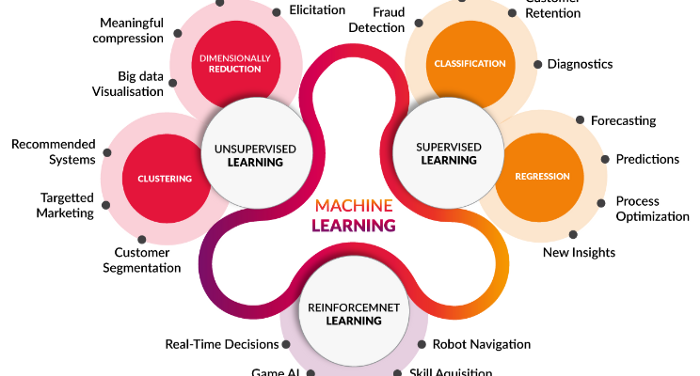
\includegraphics[width=\linewidth]{figures/mlWorld.png}
    \caption{ World of machine learning }
    \source {towardsdatascience.com}
\label{fig:mlWorld}
\end{figure}



%Machine Learning is a term that describes algorithms that learn from data.
%Goodfellow et al. quotes Mitchell from 1996 for a definition of
%what learning means, A computer program is said to learn from experience
%E with respect to some class of tasks T and performance measure P, if its
%performance at tasks in T, as measured by P, improves with experience E.
%There is a wide variety of tasks T that can be done. For instance common
%tasks are regression, classification, anomaly detection, denoising and translation.
%Depending on what experience E they see during the learning process the most
%algorithms can be classified as supervised or unsupervised learning. Supervised
%learning algorithms experience a data set together with target values or labels
%that act as instructions on what to do. The unsupervised learning algorithms
%don’t have any labels or targets but instead try to learn about the structure of
%the data set. The performance P can be how far off from the labels the output
%of the algorithm is in the case of supervised learning. This performance measure
%is often difficult to choose.




Using Machine Learning we can accomplish manly 3 of these following tasks.
\begin{itemize}
\item Regression: Regression attempts to estimate a numerical value from a given number of data points. Forecasting sharemarket or climate, financial audit, for example. There are many types of algorithms for regression analysis. Like – linear, logistic, polynomial, table, [4 in ml], etc.

\item Classification: This technique predicts that a class will be trained on a dataset with many predefined classes. For instance – a model trained on a dataset consists of photos of many animals and then predicts which animal it is when a new image is seen. Multiple types of classification can include binary classifiers, multiclass classifiers. Numerous algorithms are available there for classification. For example – Naive Baias , Decision Trees, and K-Nearest Neighbours. [5 in ml].

\item Clustering: The technology of clustering attempts to identify similarities between data points and to create new clusters with the same data points. When it comes to user behavior research, recommender systems, it is useful to show similarities between data points. For example, a data set consists of data of the customers of a business, using the clustering algorithms on the data set we can group the customer in sections which will help the business to make better decisions. Many well-known clustering algorithms such as – K-means, expectation-maximization, hierarchical, density-based, etc [6 in ml] are available.

\end{itemize}


So we can see there are many forms of machine learning, as we are using Convolutional Neural Network (CNN) withs is a type of Artificial Neural Network, we are going to discuss details about it in the upcoming sections.





\section{Artificial Neural Network}

An Artificial Neural Network usually called neural network is an artificial representation of the human brain. Basically, a neural network is a set of input/output nodes. Each node performs a simple computation by its node function. The connection among the nodes has a weight associated with it. The neural network tries to simulate its learning process.




\begin{figure}[h!]
  \centering
  \begin{subfigure}[b]{0.5\linewidth}
    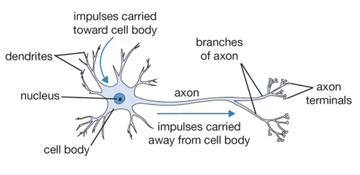
\includegraphics[width=\linewidth]{figures/bgn.png}
    \caption{Single biological neuron}
  \end{subfigure}
\quad
\begin{subfigure}[b]{0.5\linewidth}
    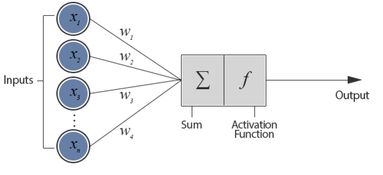
\includegraphics[width=\linewidth]{figures/ann.png}
    \caption{Mathematically modeled biological neuron}
  \end{subfigure}
 \caption{Biological neuron vs artificial neuron}
  \label{fig:bgnVSann}
  \source {datacamp.com}
\end{figure}

An Artificial Neuron tries to mimic the function of neurons in a biological brain. As a biological neuron gets some electric signal from the previous neuron from its dendrite and then passes on the signal if the signal has a certain threshold value through its axon to the next neuron. Together they form millions and billions of connections.
This function of a biological neuron can be mathematically modeled. we get some values and we use an activation function to determine the threshold and can pass it on. The figure represents the functional similarities of a biological and computer-modeled neuron.









\section{Deep Learning}
Deep Learning is a term used for training deep artificial neural networks, or
ANN s. An ANN is a function approximator consisting of multiple functions,

also called neurons. An ANN is called a feedforward ANN if there are no
feedback connections of the output of the ANN being sent to itself. Each neuron
is a linear function of some inputs, fed into a nonlinear function, called activation
function. If the input of a neuron is a vector x, the output of the neuron gi can
be written as


\subsection{Convulitional Neural Network}
The non-linear functions called activation functions, such as K in Equation 2.1,
are typically fixed non-linear functions that are used to make the ANN able to
approximate non-linear functions. If the non-linear activation functions weren’t
used, the output of the ANN would still be a linear function of the inputs x. In deep learning, there are a few commonly used functions that
have become standard as activation functions.
The rectifying linear unit, or ReLU is a function that is defined as


\subsection{Back-propagation}
When training a ANN to approximate a function, gradient based optimization
is commonly used. To compute the gradient of a (loss) function f with
respect to the parameters  an algorithm called back-propagation is commonly
used. It back-propagates from the objective function to gradients of the different
weights and biases in the ANN to compute the gradient of the objective function with respect to all the parameters. If we have a function 
can be a cost function in a supervised learning setting but could also be other
functions like a reward function in the reinforcement learning setting that will

\subsection{Gradient based optimization for deep learning}

The ANN weights and biases are updated to optimize some objective function
with gradient based optimization, using the gradients computed with the backprop algorithm.
The classic algorithm for optimizing the parameters in a ANN is called Gradient
Descent. be an objective function that we want to minimize, where
x is the input to the ANN the trainable parameters of the ANN. Then
moving in the opposite direction of the gradient of L with respect to  we move
the parameters in a direction that makes the objective function smaller, which is
what we want. However, usually x are random samples and the true gradient is
the expected value of the gradient with respect to the random samples actually
used. Thus when computing the gradient of the loss function as a function of
some samples x, we are computing an unbiased noisy estimate of the gradient.
This is referred to as Stochastic Gradient Descent, or SGD. Stochastic Gradient

\subsection{Batch Normalization}
Batch Normalization is a recent method in deep learning used to be able to train
networks faster and use higher learning rates with decreased risk of divergence.
It does so by making the normalization a part of the model architecture, fixing
the mean and variances of the inputs to a layer by a normalization step. This
makes the risk of the inputs to the activation functions getting in a range where
the gradient vanishes smaller and allows for the use of higher learning rates. 

\section{Deep Learning}
Deep Learning is a term used for training deep artificial neural networks, or
ANN s. An ANN is a function approximator consisting of multiple functions,

also called neurons. An ANN is called a feedforward ANN if there are no
feedback connections of the output of the ANN being sent to itself. Each neuron
is a linear function of some inputs, fed into a nonlinear function, called activation
function. If the input of a neuron is a vector x, the output of the neuron gi can
be written as


\subsection{Activation Functions}
The non-linear functions called activation functions, such as K in Equation 2.1,
are typically fixed non-linear functions that are used to make the ANN able to
approximate non-linear functions. If the non-linear activation functions weren’t
used, the output of the ANN would still be a linear function of the inputs x. In deep learning, there are a few commonly used functions that
have become standard as activation functions.
The rectifying linear unit, or ReLU is a function that is defined as

\subsection{Cost Functions}
To train a ANN, cost functions are usually minimized. In supervised learning, where we have labeled data to learn from, the cost functions are more
straightforward than for instance in reinforcement learning that we will discuss
in section 
The two main problems of supervised learning are regression and classification.
In regression one wants to predict a numerical value whereas in classification the
goal is to predict which class something belongs to given some inputs. Different
loss functions are common for regression and classification. Most of them are
however derived from the same principle, the one of Maximum Likelihood.

\subsection{Back-propagation}
When training a ANN to approximate a function, gradient based optimization
is commonly used. To compute the gradient of a (loss) function f with
respect to the parameters  an algorithm called back-propagation is commonly
used. It back-propagates from the objective function to gradients of the different
weights and biases in the ANN to compute the gradient of the objective function with respect to all the parameters. If we have a function 
can be a cost function in a supervised learning setting but could also be other
functions like a reward function in the reinforcement learning setting that will

\subsection{Gradient based optimization for deep learning}

The ANN weights and biases are updated to optimize some objective function
with gradient based optimization, using the gradients computed with the backprop algorithm.
The classic algorithm for optimizing the parameters in a ANN is called Gradient
Descent. be an objective function that we want to minimize, where
x is the input to the ANN the trainable parameters of the ANN. Then
moving in the opposite direction of the gradient of L with respect to  we move
the parameters in a direction that makes the objective function smaller, which is
what we want. However, usually x are random samples and the true gradient is
the expected value of the gradient with respect to the random samples actually
used. Thus when computing the gradient of the loss function as a function of
some samples x, we are computing an unbiased noisy estimate of the gradient.
This is referred to as Stochastic Gradient Descent, or SGD. Stochastic Gradient


